% !TeX program = xelatex
\documentclass[a4paper,10pt]{article}

% ============================================================================
% ១. កញ្ចប់បណ្ណាល័យ និងការកំណត់ទំព័រ (Packages & Page Setup — តាមគំរូ ls_plan.tex)
% ============================================================================
\usepackage[a4paper, left=0.95cm, right=0.95cm, top=0.85cm, bottom=0.92cm, footskip=0.52cm]{geometry}
\usepackage{amsmath}
\usepackage{unicode-math}
\usepackage{fontspec}
\usepackage{longtable, array, multirow, colortbl}
\usepackage[table]{xcolor}
\usepackage{enumitem}
\usepackage{pifont}
\usepackage{fancyhdr}
\usepackage{tikz}
\usetikzlibrary{calc, arrows.meta, decorations.pathreplacing, patterns, positioning, babel}

\makeatletter
\let\@expl@@@mark@update@singlecol@structures@@\relax
\makeatother

% --- ប្រព័ន្ធស្វែងរកទីតាំងពុម្ពអក្សរស្វ័យប្រវត្តិ (Windows Local + Cloud Repo fonts/) ---
\providecommand{\NGSFindFonts}{%
  \IfFileExists{C:/Windows/Fonts/cambria.ttc}{%
    \def\NGSSysPath{C:/Windows/Fonts/}%
    \def\NGSUserPath{C:/Users/KIT/AppData/Local/Microsoft/Windows/Fonts/}%
  }{%
    \IfFileExists{./fonts/KhmerOSsiemreap.ttf}{\def\NGSSysPath{./fonts/}\def\NGSUserPath{./fonts/}}{%
    \IfFileExists{../fonts/KhmerOSsiemreap.ttf}{\def\NGSSysPath{../fonts/}\def\NGSUserPath{../fonts/}}{%
    \IfFileExists{../../fonts/KhmerOSsiemreap.ttf}{\def\NGSSysPath{../../fonts/}\def\NGSUserPath{../../fonts/}}{%
    \IfFileExists{../../../fonts/KhmerOSsiemreap.ttf}{\def\NGSSysPath{../../../fonts/}\def\NGSUserPath{../../../fonts/}}{%
    \IfFileExists{../../../../fonts/KhmerOSsiemreap.ttf}{\def\NGSSysPath{../../../../fonts/}\def\NGSUserPath{../../../../fonts/}}{%
    \IfFileExists{../../../../../fonts/KhmerOSsiemreap.ttf}{\def\NGSSysPath{../../../../../fonts/}\def\NGSUserPath{../../../../../fonts/}}{%
    \IfFileExists{../../../../../../fonts/KhmerOSsiemreap.ttf}{\def\NGSSysPath{../../../../../../fonts/}\def\NGSUserPath{../../../../../../fonts/}}{%
      \def\NGSSysPath{../../../../../../../fonts/}\def\NGSUserPath{../../../../../../../fonts/}%
    }}}}}}}%
  }%
}
\NGSFindFonts

% ============================================================================
% ២. កំណត់ពុម្ពអក្សរ (Fonts — តាមគំរូ ls_plan.tex)
% ============================================================================
\setmathfont[Path={\NGSSysPath}, FontIndex=1, Scale=1.02]{cambria.ttc}
\defaultfontfeatures{Ligatures=TeX}

\setmainfont[
  Path={\NGSUserPath},
  Extension=.ttf,
  Script=Khmer,
  BoldFont={KhmerOSsiemreap},
  BoldFeatures={FakeBold=1.8},
  ItalicFont={KhmerOSsiemreap},
  ItalicFeatures={FakeSlant=0.25},
  BoldItalicFont={KhmerOSsiemreap},
  BoldItalicFeatures={FakeBold=1.8, FakeSlant=0.25}
]{KhmerOSsiemreap}

\newfontfamily\muol[Path={\NGSUserPath}, Extension=.ttf, Script=Khmer]{KhmerOSmuollight}
\newfontfamily\Tacteing[Path={\NGSUserPath}, Extension=.TTF]{TACTENG}
\newfontfamily\TimesEn[Path={\NGSSysPath}, Extension=.ttf, BoldFont={timesbd}, ItalicFont={timesi}, BoldItalicFont={timesbi}]{times}
\newfontfamily\CalibriFont[Path={\NGSSysPath}, Extension=.ttf]{calibri}
\newfontfamily\CourierCirc[Path={\NGSSysPath}, Extension=.ttf]{cour}

\XeTeXlinebreaklocale "km"
\XeTeXlinebreakskip = 0pt plus 1pt minus 0.1pt

% ============================================================================
% ៣. ពណ៌ និងការតុបតែង (Colors & Styles)
% ============================================================================
\definecolor{stepbg}{HTML}{D9D9D9}
\definecolor{headgray}{HTML}{E6E6E6}
\definecolor{emphred}{HTML}{C00000}

\pagestyle{fancy}
\fancyhf{}
\renewcommand{\headrulewidth}{0pt}
\fancyfoot[R]{\CalibriFont\fontsize{9pt}{11pt}\selectfont\thepage}

\setlength{\parindent}{0pt}
\setlength{\parskip}{0pt}
\setlength{\tabcolsep}{4.5pt}
\setlength{\LTpre}{2pt}
\setlength{\LTpost}{2pt}

\newcolumntype{L}[1]{>{\raggedright\arraybackslash}p{#1}}
\newcolumntype{C}[1]{>{\centering\arraybackslash}p{#1}}

% ============================================================================
% ៤. ពាក្យបញ្ជាជំនួយ (Helper Macros)
% ============================================================================
\newcommand{\en}[1]{{\TimesEn #1}}
\newcommand{\enbf}[1]{{\TimesEn\bfseries #1}}
\newcommand{\khmflourish}{{\Tacteing\fontsize{15pt}{15pt}\selectfont 3}}
\newcommand{\wcirc}{{\CourierCirc\fontsize{9.5pt}{11pt}\selectfont o}}
\newcommand{\ditem}{{\fontsize{7.5pt}{10pt}\selectfont\ding{117}}\ }
\newcommand{\fiveE}[1]{\textcolor{emphred}{\CalibriFont\bfseries #1}}
\newcommand{\redsub}[1]{\textcolor{emphred}{#1}}
\newcommand{\timenote}[1]{\textcolor{emphred}{\textit{#1}}}
\newcommand{\stepheader}[1]{\multicolumn{3}{|c|}{\cellcolor{stepbg}\muol #1} \\ \hline}
\newcommand{\cfig}[1]{{\centering\vspace{3pt}#1\vspace{3pt}\par}}
\newcommand{\cnum}[1]{\mbox{\fontsize{10.5pt}{12pt}\selectfont\ding{\numexpr181+#1\relax}}}
\newcommand{\unit}[1]{\,\text{\en{#1}}}
\newcommand{\riel}{\,\text{៛}}
\newcommand{\graybox}[1]{\colorbox{headgray}{\strut #1}}

% ============================================================================
% ៥. រូបភាព TikZ ស-ខ្មៅ សម្រាប់បង្រៀនលើក្ដារខៀន និងសន្លឹកកិច្ចការ (B&W Diagrams)
% ============================================================================

% ១. E1 Engage: អន្ទាក់ការេនៃផលបូក (x + 3)^2 = x^2 + 9 vs x^2 + 6x + 9
\newcommand{\figEngageALGFiveFive}{%
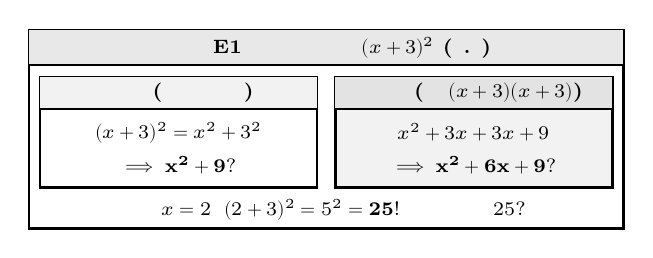
\begin{tikzpicture}[x=1cm, y=1cm, every node/.style={font=\scriptsize, text=black}]
  \draw[black, line width=0.9pt] (0,0) rectangle (7.55,2.52);
  \fill[gray!18] (0,2.08) rectangle (7.55,2.52);
  \draw[black, line width=0.6pt] (0,2.08) -- (7.55,2.08);
  \node at (3.775,2.30) {\textbf{បេសកកម្ម \en{E1}៖ ពន្លាតការេនៃទ្វេធា $(x + 3)^2$ (ទំ.៦៣)}};

  % Student A
  \draw[black, line width=0.8pt] (0.14,0.52) rectangle (3.66,1.92);
  \fill[gray!10] (0.14,1.52) rectangle (3.66,1.92);
  \draw[black, line width=0.5pt] (0.14,1.52) -- (3.66,1.52);
  \node at (1.90,1.72) {\textbf{សិស្ស ក (លើកការេដាច់គ្នា)}};
  \node at (1.90,1.22) {$(x+3)^2 = x^2 + 3^2$};
  \node at (1.90,0.80) {$\implies \mathbf{x^2 + 9}$?};

  % Student B
  \draw[black, line width=0.95pt, fill=gray!10] (3.89,0.52) rectangle (7.41,1.92);
  \fill[gray!22] (3.89,1.52) rectangle (7.41,1.92);
  \draw[black, line width=0.55pt] (3.89,1.52) -- (7.41,1.52);
  \node at (5.65,1.72) {\textbf{សិស្ស ខ (គុណ $(x+3)(x+3)$)}};
  \node at (5.65,1.22) {$x^2 + 3x + 3x + 9$};
  \node at (5.65,0.80) {$\implies \mathbf{x^2 + 6x + 9}$?};

  \node at (3.775,0.24) {\textbf{តេស្ត $x = 2$៖} $(2+3)^2 = 5^2 = \mathbf{25}$! តើកន្សោមណាស្មើ $25$?};
\end{tikzpicture}}

% ២. E2 Explore: គំរូផ្ទៃការេជ្រុង a+b និងការគណនា (a-b)(a+b) (ទំ.៦៣--៦៥)
\newcommand{\figExploreALGFiveFive}{%
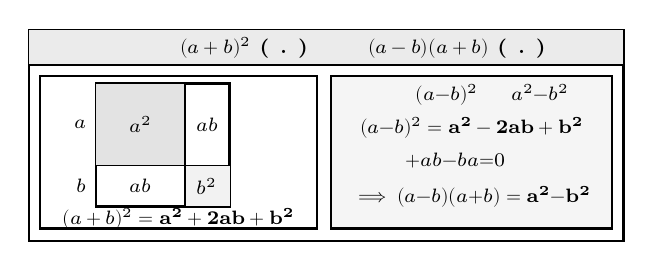
\begin{tikzpicture}[x=1cm, y=1cm, every node/.style={font=\scriptsize, text=black}]
  \draw[black, line width=0.9pt] (0,0) rectangle (7.55,2.68);
  \fill[gray!16] (0,2.24) rectangle (7.55,2.68);
  \draw[black, line width=0.6pt] (0,2.24) -- (7.55,2.24);
  \node at (3.775,2.46) {\textbf{គំរូផ្ទៃការេ $(a+b)^2$ (ទំ.៦៣) និងផលគុណ $(a-b)(a+b)$ (ទំ.៦៥)}};

  % Left: Square of side a + b
  \draw[black, line width=0.8pt] (0.14,0.16) rectangle (3.66,2.10);
  \draw[black, line width=0.9pt] (0.85,0.44) rectangle (2.55,2.00);
  \fill[gray!22] (0.85,0.96) rectangle (1.98,2.00);
  \fill[gray!10] (1.98,0.44) rectangle (2.55,0.96);
  \draw[black, line width=0.65pt] (1.98,0.44) -- (1.98,2.00);
  \draw[black, line width=0.65pt] (0.85,0.96) -- (2.55,0.96);
  \node at (0.66,1.48) {$a$};
  \node at (0.66,0.70) {$b$};
  \node at (1.42,1.48) {$a^2$};
  \node at (2.26,1.48) {$ab$};
  \node at (1.42,0.70) {$ab$};
  \node at (2.26,0.70) {$b^2$};
  \node at (1.90,0.28) {$(a+b)^2 = \mathbf{a^2 + 2ab + b^2}$};

  % Right: (a-b)^2 and (a-b)(a+b)
  \draw[black, line width=0.8pt, fill=gray!8] (3.84,0.16) rectangle (7.41,2.10);
  \node at (5.625,1.86) {\textbf{ពន្លាត $(a{-}b)^2$ និង $a^2{-}b^2$}};
  \node at (5.625,1.44) {$(a{-}b)^2 = \mathbf{a^2 - 2ab + b^2}$};
  \node at (5.625,1.02) {តួ $+ab{-}ba{=}0$ ស៊ីសងអស់};
  \node at (5.625,0.56) {$\implies (a{-}b)(a{+}b) = \mathbf{a^2{-}b^2}$};
\end{tikzpicture}}

% ៣. E3 Explain: សង្ខេបរូបមន្តសមភាពសំខាន់ៗ (1), (2), (3)
\newcommand{\figRuleALGFiveFive}{%
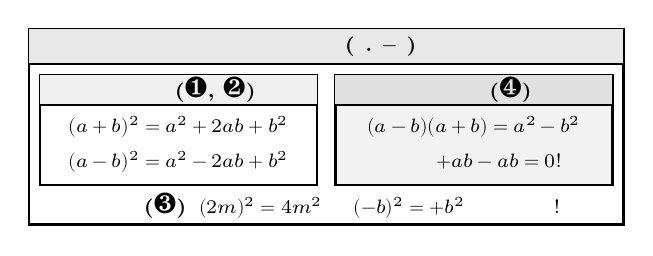
\begin{tikzpicture}[x=1cm, y=1cm, every node/.style={font=\scriptsize, text=black}]
  \draw[black, line width=0.9pt] (0,0) rectangle (7.55,2.48);
  \fill[gray!18] (0,2.04) rectangle (7.55,2.48);
  \draw[black, line width=0.6pt] (0,2.04) -- (7.55,2.04);
  \node at (3.775,2.26) {\textbf{សមភាពសំខាន់ៗទាំង ៣ (ទំ.៦៣--៦៥)}};

  % Left: Square of binomial
  \draw[black, line width=0.8pt] (0.14,0.50) rectangle (3.66,1.90);
  \fill[gray!12] (0.14,1.52) rectangle (3.66,1.90);
  \draw[black, line width=0.55pt] (0.14,1.52) -- (3.66,1.52);
  \node at (1.90,1.71) {\textbf{ការេនៃទ្វេធា (\cnum{1}, \cnum{2})}};
  \node at (1.90,1.24) {$(a+b)^2 = a^2 + 2ab + b^2$};
  \node at (1.90,0.80) {$(a-b)^2 = a^2 - 2ab + b^2$};

  % Right: Product of sum and difference
  \draw[black, line width=0.95pt, fill=gray!10] (3.89,0.50) rectangle (7.41,1.90);
  \fill[gray!24] (3.89,1.52) rectangle (7.41,1.90);
  \draw[black, line width=0.6pt] (3.89,1.52) -- (7.41,1.52);
  \node at (5.65,1.71) {\textbf{ផលបូកគុណផលដក (\cnum{4})}};
  \node at (5.65,1.24) {$(a-b)(a+b) = a^2 - b^2$};
  \node at (5.65,0.80) {តួកណ្ដាល $+ab - ab = 0$!};

  \node at (3.775,0.24) {\textbf{ប្រយ័ត្ន (\cnum{3})៖} $(2m)^2 = 4m^2$ និង $(-b)^2 = +b^2$ វិជ្ជមានជានិច្ច!};
\end{tikzpicture}}

% ៤. E4 Elaborate: លំហាត់គំរូពន្លាតមេគុណ និងមុធាគណនារហ័ស (ទំ.៦៤--៦៥)
\newcommand{\figElaborateALGFiveFive}{%
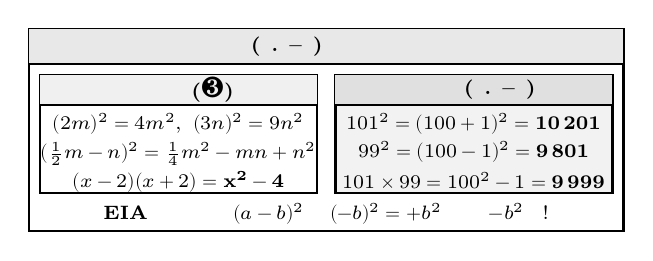
\begin{tikzpicture}[x=1cm, y=1cm, every node/.style={font=\scriptsize, text=black}]
  \draw[black, line width=0.9pt] (0,0) rectangle (7.55,2.56);
  \fill[gray!18] (0,2.12) rectangle (7.55,2.56);
  \draw[black, line width=0.6pt] (0,2.12) -- (7.55,2.12);
  \node at (3.775,2.34) {\textbf{លំហាត់គំរូ (ទំ.៦៤--៦៥)៖ មេគុណទ្វេធា និងមុធាគណនា}};

  % Left: Algebraic terms
  \draw[black, line width=0.8pt] (0.14,0.48) rectangle (3.66,1.98);
  \fill[gray!12] (0.14,1.60) rectangle (3.66,1.98);
  \draw[black, line width=0.55pt] (0.14,1.60) -- (3.66,1.60);
  \node at (1.90,1.79) {\textbf{ពន្លាតមេគុណ (\cnum{3})}};
  \node at (1.90,1.36) {$(2m)^2 = 4m^2, \ (3n)^2 = 9n^2$};
  \node at (1.90,0.98) {$(\tfrac{1}{2}m-n)^2 = \tfrac{1}{4}m^2-mn+n^2$};
  \node at (1.90,0.62) {$(x-2)(x+2) = \mathbf{x^2 - 4}$};

  % Right: Mental math
  \draw[black, line width=0.95pt, fill=gray!10] (3.89,0.48) rectangle (7.41,1.98);
  \fill[gray!24] (3.89,1.60) rectangle (7.41,1.98);
  \draw[black, line width=0.6pt] (3.89,1.60) -- (7.41,1.60);
  \node at (5.65,1.79) {\textbf{មុធាគណនា (ទំ.៦៤--៦៥)}};
  \node at (5.65,1.36) {$101^2 = (100+1)^2 = \mathbf{10\,201}$};
  \node at (5.65,1.00) {$99^2 = (100-1)^2 = \mathbf{9\,801}$};
  \node at (5.65,0.64) {$101\times 99 = 100^2 - 1 = \mathbf{9\,999}$};

  \node at (3.775,0.22) {\textbf{\en{EIA}៖} តួចុងក្រោយនៃ $(a-b)^2$ គឺ $(-b)^2 = +b^2$ មិនមែន $-b^2$ ទេ!};
\end{tikzpicture}}

% ៥. E5 Evaluate: ជម្រើសវិនិច្ឆ័យ A-D ពន្លាត (3x - 2y)^2
\newcommand{\figExitALGFiveFive}{%
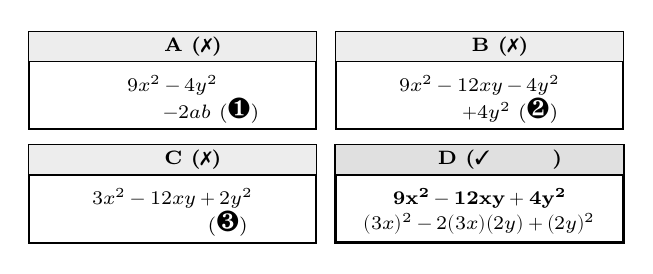
\begin{tikzpicture}[x=1cm, y=1cm, every node/.style={font=\scriptsize, text=black}]
  % Choice A
  \draw[black, line width=0.8pt] (0,1.44) rectangle (3.65,2.68);
  \fill[gray!14] (0,2.30) rectangle (3.65,2.68);
  \draw[black, line width=0.5pt] (0,2.30) -- (3.65,2.30);
  \node at (1.825,2.49) {\textbf{ជម្រើស \en{A} (\ding{55})}};
  \node at (1.825,2.00) {$9x^2 - 4y^2$};
  \node at (1.825,1.68) {ភ្លេចតួកណ្ដាល $-2ab$ (\cnum{1})};

  % Choice B
  \draw[black, line width=0.8pt] (3.90,1.44) rectangle (7.55,2.68);
  \fill[gray!14] (3.90,2.30) rectangle (7.55,2.68);
  \draw[black, line width=0.5pt] (3.90,2.30) -- (7.55,2.30);
  \node at (5.725,2.49) {\textbf{ជម្រើស \en{B} (\ding{55})}};
  \node at (5.725,2.00) {$9x^2 - 12xy - 4y^2$};
  \node at (5.725,1.68) {ខុសសញ្ញាតួ $+4y^2$ (\cnum{2})};

  % Choice C
  \draw[black, line width=0.8pt] (0,0) rectangle (3.65,1.24);
  \fill[gray!14] (0,0.86) rectangle (3.65,1.24);
  \draw[black, line width=0.5pt] (0,0.86) -- (3.65,0.86);
  \node at (1.825,1.05) {\textbf{ជម្រើស \en{C} (\ding{55})}};
  \node at (1.825,0.56) {$3x^2 - 12xy + 2y^2$};
  \node at (1.825,0.24) {ភ្លេចលើកមេគុណជាការេ (\cnum{3})};

  % Choice D (Correct)
  \draw[black, line width=1.05pt] (3.90,0) rectangle (7.55,1.24);
  \fill[gray!24] (3.90,0.86) rectangle (7.55,1.24);
  \draw[black, line width=0.6pt] (3.90,0.86) -- (7.55,0.86);
  \node at (5.725,1.05) {\textbf{ជម្រើស \en{D} (\ding{51} ត្រឹមត្រូវ)}};
  \node at (5.725,0.56) {$\mathbf{9x^2 - 12xy + 4y^2}$};
  \node at (5.725,0.24) {$(3x)^2 - 2(3x)(2y) + (2y)^2$};
\end{tikzpicture}}

\begin{document}
\fontsize{10pt}{15.2pt}\selectfont

% ============================================================================
% ក្បាលរដ្ឋបាល (Administrative Header — តាមគំរូ ls_plan.tex)
% ============================================================================
{\centering
  {\muol\fontsize{11pt}{16pt}\selectfont ព្រះរាជាណាចក្រកម្ពុជា\par}
  {\muol\fontsize{11pt}{16pt}\selectfont ជាតិ សាសនា ព្រះមហាក្សត្រ\par}
  \vspace{-3pt}{\khmflourish\par}
}

\vspace{1pt}
{\muol\fontsize{10pt}{15.5pt}\selectfont
មន្ទីរអប់រំ យុវជន និងកីឡា ខេត្តកំពង់ធំ\par
ការិយាល័យអប់រំ យុវជន និងកីឡា ស្រុកកំពង់ស្វាយ\par
អនុវិទ្យាល័យព្រះក្រសាំង\par}

\vspace{2pt}
{\centering{\muol\fontsize{11.5pt}{17pt}\selectfont កិច្ចតែងការបង្រៀន\par}}
\vspace{2pt}

% --- ព័ត៌មានទូទៅ ---
{\hspace*{2.8cm}\renewcommand{\arraystretch}{1.08}
\begin{tabular}{@{}l@{\hspace{0.35cm}}p{2.9cm}@{\hspace{0.15cm}}c@{\hspace{0.25cm}}l@{}}
  - & មុខវិជ្ជា & : & គណិតវិទ្យា ថ្នាក់ទី៨ (ពីជគណិត) \\
  - & ចំណងជើងមេរៀន & : & មេរៀនទី៥៖ កន្សោមពីជគណិត \\
  - & ចំណងជើងរង & : & ៣.១ ពន្លាតការេនៃទ្វេធា និងផលគុណនៃផលបូកនិងផលដកពីរចំនួន \\
  - & រយៈពេល & : & ១ ម៉ោងសិក្សា (៥០ នាទី) \\
  - & បង្រៀនដោយ & : & ហុក ប៊ុនថែន \\
  - & កាលបរិច្ឆេទ & : & ថ្ងៃពុធ ទី៩ ខែធ្នូ ឆ្នាំ២០២៦ \\
\end{tabular}\par}

\vspace{2pt}

% --- I. វត្ថុបំណង ---
{\muol\fontsize{10pt}{15.5pt}\selectfont \enbf{I.} វត្ថុបំណង\par}
\vspace{1pt}
{\renewcommand{\arraystretch}{1.10}
\begin{tabular}{@{}p{0.55cm}@{}p{2.35cm}@{\hspace{0.15cm}}c@{\hspace{0.25cm}}p{14.95cm}@{}}
  \hfill\wcirc\hspace{0.2cm} & វិជ្ជាសម្បទា & : & សិស្សប្រាប់រូបមន្តសមភាពសំខាន់ៗទាំង ៣ គឺ $(a+b)^2 = a^2+2ab+b^2$, $(a-b)^2 = a^2-2ab+b^2$ និង $(a-b)(a+b) = a^2-b^2$ បានត្រឹមត្រូវ (ទំ.៦៣--៦៥) ។ \\
  \hfill\wcirc\hspace{0.2cm} & បំណិនសម្បទា & : & សិស្សប្រើសមភាពសំខាន់ៗទាំង ៣ ដើម្បីពន្លាតកន្សោមពីជគណិត និងមុធាគណនាលេខរហ័សលើសន្លឹកកិច្ចការបានត្រឹមត្រូវ ។ \\
  \hfill\wcirc\hspace{0.2cm} & ចរិយាសម្បទា & : & សិស្សមានទម្លាប់ផ្ទៀងផ្ទាត់តួកណ្ដាល $\pm 2ab$ និងលើកមេគុណជាការេដោយប្រុងប្រយ័ត្ន មិនច្រឡំតាមភាពលីនេអ៊ែរក្លែងក្លាយ ។ \\
\end{tabular}\par}

\vspace{2pt}

% --- II. សម្ភារៈឧបទេស ---
{\muol\fontsize{10pt}{15.5pt}\selectfont \enbf{II.} សម្ភារៈឧបទេស\par}
\vspace{1pt}
\hspace*{0.55cm}$\bullet$\ សៀវភៅសិក្សាគោលថ្នាក់ទី៨ (ទំ.៦៣--៦៦, ៧៣) ក្ដារខៀន ដីស/ហ្វឺត បន្ទាត់ត្រង់ និង\textbf{សន្លឹកកិច្ចការសិស្សបំពេញចន្លោះ ស-ខ្មៅ} (កូដ \en{ALG55} ទំព័រ ១--២ សម្រាប់សិស្ស និងទំព័រ ៣ ប្លង់ក្ដារខៀន/ចម្លើយគ្រូ — គ្មានប្រើ \en{LCD})\par

\vspace{2pt}

% --- III. វិធីសាស្រ្តបង្រៀន ---
{\muol\fontsize{10pt}{15.5pt}\selectfont \enbf{III.} វិធីសាស្រ្តបង្រៀន\par}
\vspace{1pt}
{\renewcommand{\arraystretch}{1.08}
\begin{tabular}{@{}p{0.55cm}@{}p{2.35cm}@{\hspace{0.15cm}}c@{\hspace{0.25cm}}p{14.95cm}@{}}
  \hfill$\bullet$\hspace{0.2cm} & គោលវិធី & : & សិស្សមជ្ឈមណ្ឌល (សន្លឹកកិច្ចការបំពេញចន្លោះជាគោល + ការពិភាក្សាជាក្រុមតូច ៣ នាក់) \\
  \hfill$\bullet$\hspace{0.2cm} & យុទ្ធវិធីបង្រៀន & : & គំរូស្ថាបនានិយម \en{5Es} រួមបញ្ចូល \textbf{ការបំបែកអន្ទាក់ភាពលីនេអ៊ែរតាមគំរូផ្ទៃការេ} និង \textbf{មុធាគណនារហ័សតាមសមភាពសំខាន់ៗ} \\
\end{tabular}\par}

\vspace{2pt}

% --- IV. ដំណើរការបង្រៀន ---
{\muol\fontsize{10pt}{15.5pt}\selectfont \enbf{IV.} ដំណើរការបង្រៀន\par}

{\renewcommand{\arraystretch}{1.15}
\begin{longtable}{|L{5.50cm}|L{7.90cm}|L{4.80cm}|}
\hline
\multicolumn{1}{|c|}{\cellcolor{headgray}\muol សកម្មភាពគ្រូ} &
\multicolumn{1}{c|}{\cellcolor{headgray}\muol ខ្លឹមសារមេរៀន} &
\multicolumn{1}{c|}{\cellcolor{headgray}\muol សកម្មភាពសិស្ស} \\
\hline
\endfirsthead

\hline
\multicolumn{1}{|c|}{\cellcolor{headgray}\muol សកម្មភាពគ្រូ} &
\multicolumn{1}{c|}{\cellcolor{headgray}\muol ខ្លឹមសារមេរៀន} &
\multicolumn{1}{c|}{\cellcolor{headgray}\muol សកម្មភាពសិស្ស} \\
\hline
\endhead

% ==================== ជំហានទី១ (2min) ====================
\stepheader{ជំហានទី១ \enbf{(}រដ្ឋបាលថ្នាក់\enbf{)}}
$\bullet$ ពិនិត្យវត្តមាន អនាម័យ និងសណ្ដាប់ធ្នាប់ថ្នាក់រៀន \par
$\bullet$ រៀបចំក្រុមតូច ៣ នាក់ និងចែក\textbf{សន្លឹកកិច្ចការសិស្ស (\en{ALG55} ទំព័រ ១–២)}
&
$\bullet$ រដ្ឋបាលថ្នាក់ អនាម័យ និងវិន័យសិក្សា \par
$\bullet$ ចែកសន្លឹកកិច្ចការម្នាក់ ១ សន្លឹក សម្រាប់បំពេញតាមដំណាក់កាល \en{E1--E5}
&
$\circ$ ប្រធានថ្នាក់រាយការណ៍វត្តមានសិស្ស \par
$\circ$ ទទួលសន្លឹកកិច្ចការ សរសេរឈ្មោះ និងអង្គុយតាមក្រុម ៣ នាក់ \\
\hline

% ==================== ជំហានទី២ (9min: កំណែ <=3m + រំលឹក 3m + E1 3m) ====================
\stepheader{ជំហានទី២ \enbf{(}កិច្ចការផ្ទះ \enbf{+} ទំនាក់ទំនងមេរៀនថ្មី\enbf{)}}
\ditem \textbf{កំណែកិច្ចការផ្ទះ ($\le\text{\enbf{3\,min}}$)} \par
$\bullet$ ហៅសិស្ស ២ នាក់ឡើងកែលំហាត់ទំ.៦០, ៦២ និងទំ.៧៣ \#6 លើក្ដារខៀន
&
{\centering\redsub{កំណែកិច្ចការផ្ទះ (ទំ.៦០, ៦២ និង ទំ.៧២–៧៣ \#2, \#6)}\par}
$\bullet$ \textbf{ទំ.៦០ (គ)៖} $\mathbf{a^3+a^2b-2ab^2}$; \ \textbf{ទំ.៦២ (ខ)៖} $\mathbf{5y^2+2xy^3-12}$; \ \textbf{(ឃ)៖} $\mathbf{a+11}$ \par
$\bullet$ \textbf{\#2៖} $1997 = 1\cdot 10^3+9\cdot 10^2+9\cdot 10+7$; \ \textbf{\#6៖} $\mathbf{2ax + 2bx - 2ab}$
&
$\circ$ ផ្ទៀងចម្លើយ និងកែតម្រូវចូលសៀវភៅកិច្ចការផ្ទះ \\[3pt]

\ditem \textbf{រំលឹកមេរៀនទាក់ទង (\enbf{3min})} \par
$\bullet$ សួរ៖ «តើ $(2m)^2$ និង $(-b)^2$ ស្មើប៉ុន្មាន? ចុះអត្ថន័យនៃ $A^2$ គឺស្មើផលគុណអ្វី?»
&
{\centering\redsub{រំលឹកការេនៃឯកធា និងនិយមន័យស្វ័យគុណទី ២}\par}
$\bullet$ $(2m)^2 = \mathbf{4m^2}$, \quad $(-b)^2 = (-b)(-b) = \mathbf{+b^2}$ \par
$\bullet$ និយមន័យ៖ $A^2 = A \times A$
&
$\circ$ ឆ្លើយ៖ «$4m^2$; $+b^2$; និង $A \times A$!» \\[3pt]

\fiveE{E1 - Engage (3min)} \timenote{(កុំទាន់ផ្ដល់ចម្លើយ)} \par
\ditem \textbf{បេសកកម្មអន្ទាក់ការេនៃផលបូក (សន្លឹកកិច្ចការ \en{E1})} \par
$\bullet$ ឱ្យសិស្សអានប្រអប់ \en{E1} ហើយតេស្តដោយជំនួស $x = 2$ ដើម្បីជ្រើសរើសរវាង\textbf{សិស្ស ក} និង\textbf{សិស្ស ខ}
&
\redsub{បេសកកម្ម \en{E1}៖ ពន្លាតការេនៃទ្វេធា $(x + 3)^2$ (ទំ.៦៣)} \par
$\bullet$ \textbf{សិស្ស ក} លើកការេដាច់គ្នា បាន $x^2 + 3^2 = x^2 + 9$! \par
$\bullet$ \textbf{សិស្ស ខ} គុណ $(x+3)(x+3)$ បាន $x^2 + 6x + 9$! តើអ្នកណាត្រូវ?
&
$\circ$ ជំនួស $x=2$ ពិភាក្សាជាគូ និងគូស \ding{51} ក្នុងប្រអប់ \en{E1} \\[3pt]

&
\cfig{\figEngageALGFiveFive}
& \\
\hline

% ==================== ជំហានទី៣ (17min: E2 11m + E3 6m) ====================
\stepheader{ជំហានទី៣ \enbf{(}ខ្លឹមសារមេរៀនថ្មី\enbf{)}}
\fiveE{E2 - Explore (11min)} \par
$\bullet$ សរសេរចំណងជើងរង \textbf{៣. សមភាពសំខាន់ៗ — ៣.១ ការេនៃទ្វេធា និង $(a-b)(a+b)$} \par
\ditem \textbf{សកម្មភាព ១៖ ការេនៃផលបូក និងការេនៃផលដក (ទំ.៦៣–៦៤, \enbf{6min}, \en{E2-A})} \par
$\bullet$ ឱ្យសិស្សបំពេញផ្ទៃក្រឡាការេជ្រុង $a+b$ និងពន្លាត $(a-b)(a-b)$ លើ \en{E2-A}
&
៣. សមភាពសំខាន់ៗ — ៣.១ ពន្លាតការេនៃទ្វេធា (ទំ.៦៣–៦៤) \par
$\bullet$ \textbf{ការេនៃផលបូក៖} $(a+b)^2 = (a+b)(a+b) = a^2 + ab + ba + b^2 = \mathbf{a^2 + 2ab + b^2}$ \par
$\bullet$ \textbf{ការេនៃផលដក៖} $(a-b)^2 = (a-b)(a-b) = a^2 - ab - ba + b^2 = \mathbf{a^2 - 2ab + b^2}$ (ឧ. $(x-1)^2 = x^2 - 2x + 1$)
&
$\circ$ បំពេញផ្ទៃការេទាំង ៤ ផ្នែក និងទាញរូបមន្ត $(a\pm b)^2$ លើ \en{E2-A} \\[3pt]

\ditem \textbf{សកម្មភាព ២៖ ផលគុណ $(a-b)(a+b)$ និងកំសាន្តគណិតវិទ្យា (ទំ.៦៥–៦៦, \enbf{5min}, \en{E2-B})} \par
$\bullet$ ឱ្យសិស្សពន្លាត $(a-b)(a+b)$ និងរកលំនាំកំសាន្តគណិតវិទ្យាទំ.៦៦ លើ \en{E2-B}
&
ផលគុណនៃផលបូកនិងផលដកពីរចំនួន (ទំ.៦៥–៦៦) \par
$\bullet$ \textbf{ពន្លាត $(a-b)(a+b)$៖} $a^2 + ab - ba - b^2 = \mathbf{a^2 - b^2}$ (ឧ. $(x-2)(x+2) = x^2 - 4$) \par
$\bullet$ \textbf{កំសាន្តគណិតវិទ្យា (ទំ.៦៦)៖} $(2+1)(2-1)=3, \ (3+2)(3-2)=5, \ (4+3)(4-3)=\mathbf{7}, \dots, (10+9)(10-9)=\mathbf{19}$
&
$\circ$ សង្កេតតួ $+ab-ab=0$ និងបំពេញលំនាំចំនួនសេសលើ \en{E2-B} \\[3pt]

&
\cfig{\figExploreALGFiveFive}
& \\[3pt]

% --- E3 Explain (6min) ---
\fiveE{E3 - Explain (6min)} \par
$\bullet$ ដឹកនាំសិស្សសង្ខេបរូបមន្តសមភាពសំខាន់ៗទី (1), (2) និង (3) (ទំ.៦៣–៦៥)
&
$\bullet$ \textbf{សមភាពសំខាន់ៗទាំង ៣ (ទំ.៦៣–៦៥)៖} \par
\hspace*{0.15cm}(1) \textbf{ការេនៃផលបូក៖} $(a + b)^2 = \graybox{$a^2 + 2ab + b^2$}$ \par
\hspace*{0.15cm}(2) \textbf{ការេនៃផលដក៖} $(a - b)^2 = \graybox{$a^2 - 2ab + b^2$}$ \par
\hspace*{0.15cm}(3) \textbf{ផលគុណផលដកនិងផលបូក៖} $(a - b)(a + b) = \graybox{$a^2 - b^2$}$
&
$\circ$ បំពេញប្រអប់រូបមន្តសមភាពសំខាន់ៗទាំង ៣ លើ \en{E3} \\[3pt]

$\bullet$ ភ្ជាប់\textbf{ធនាគារហេតុផល \cnum{1}--\cnum{4}} លើក្ដារខៀន និងសន្លឹកកិច្ចការ
&
\textbf{ធនាគារហេតុផល (\en{Warrant Bank})៖} \par
\cnum{1} \textbf{តួកណ្ដាល $\pm 2ab$៖} ការេនៃទ្វេធា $(a\pm b)^2$ ត្រូវមាន $3$ តួជានិច្ច (ហាមភ្លេច $\pm 2ab$) \par
\cnum{2} \textbf{តួចុងក្រោយ $+b^2$៖} ទាំង $(a+b)^2$ ទាំង $(a-b)^2$ មានតួចុងក្រោយ $+b^2$ វិជ្ជមានជានិច្ច
&
$\circ$ ផ្ទៀងលេខកូដ \cnum{1}--\cnum{2} លើសន្លឹកកិច្ចការ \\[3pt]

&
\cnum{3} \textbf{ការេនៃមេគុណ៖} ពេលពន្លាត $(2m+3n)^2$ ត្រូវលើកមេគុណជាការេ $(2m)^2 = 4m^2$ \par
\cnum{4} \textbf{កន្សោមឆ្លាស់៖} $(a-b)(a+b) = a^2 - b^2$ ស៊ីសងតួកណ្ដាលអស់ នៅសល់តែផលដកពីរការេ
&
$\circ$ ផ្ទៀងលេខកូដ \cnum{3}--\cnum{4} លើសន្លឹកកិច្ចការ \\[3pt]

&
\cfig{\figRuleALGFiveFive}
& \\
\hline

% ==================== ជំហានទី៤ (20min: E4 10m + E5 10m) ====================
\stepheader{ជំហានទី៤ \enbf{(}ពង្រីកចំណេះដឹង\enbf{)}}
\fiveE{E4 - Elaborate (10min)} \par
\ditem \textbf{លំហាត់គំរូ៖ ពន្លាតទ្វេធាមានមេគុណ និងមុធាគណនា (ទំ.៦៤–៦៥)} \par
$\bullet$ ឱ្យសិស្សធ្វើលំហាត់គំរូទំ.៦៤–៦៥ ទាំងកន្សោមអថេរ និងលេខរហ័សលើ \en{E4}
&
{\muol លំហាត់គំរូ} \textbf{(ទំ.៦៤–៦៥)៖} \par
$\bullet$ \textbf{១) ពន្លាតកន្សោមមានមេគុណ និងប្រភាគ៖} \par
\hspace*{0.2cm}-- $(2m+3n)^2 = (2m)^2+2(2m)(3n)+(3n)^2 = \graybox{$4m^2+12mn+9n^2$}$ \par
\hspace*{0.2cm}-- $(\tfrac{1}{2}m-n)^2 = \mathbf{\tfrac{1}{4}m^2 - mn + n^2}$; \quad $(\tfrac{1}{2}m-3n)(\tfrac{1}{2}m+3n) = \mathbf{\tfrac{1}{4}m^2 - 9n^2}$ \par
$\bullet$ \textbf{២) មុធាគណនារហ័ស (ទំ.៦៤–៦៥)៖} \par
\hspace*{0.2cm}-- $101^2 = (100+1)^2 = \mathbf{10\,201}$; \quad $99^2 = (100-1)^2 = \mathbf{9\,801}$ \par
\hspace*{0.2cm}-- $101 \times 99 = (100+1)(100-1) = 10\,000 - 1 = \graybox{$9\,999$}$
&
$\circ$ ពន្លាតកន្សោម និងគណនាលេខរហ័សលើ \en{E4} ត្រឹមត្រូវ \\[3pt]

&
\cfig{\figElaborateALGFiveFive}
& \\[3pt]

$\bullet$ សួរសំណួរឆ្លុះបញ្ចាំង \textbf{\en{EIA Looking-Back} (1min)}
&
\textbf{\en{EIA Looking-Back}៖} «ហេតុអ្វី $(a-b)^2$ ស្មើនឹង $(b-a)^2$?» ($\to$ ព្រោះ $(b-a)^2 = b^2 - 2ba + a^2 = a^2 - 2ab + b^2 = (a-b)^2$ ចំនួនផ្ទុយគ្នាលើកជាការេស្មើគ្នា!)
&
$\circ$ ពន្យល់ថា $(-X)^2 = X^2$ ដូច្នេះ $(a-b)^2 = (b-a)^2$ \\[3pt]

% --- E5 Evaluate (10min) ---
\fiveE{E5 - Evaluate (10min)} \par
\ditem \textbf{ប្រតិបត្តិជាក្រុមតូច ៣ នាក់ (4min, សន្លឹកកិច្ចការ \en{E5})} \par
$\bullet$ ឱ្យសិស្សដោះស្រាយប្រតិបត្តិទំ.៦៤ (ក) និងទំ.៦៥ (ក, គ)
&
{\muol លំហាត់ប្រតិបត្តិ} \textbf{(ទំ.៦៤–៦៥)៖} \par
$\bullet$ \textbf{១) ទំ.៦៤ (ក) និង ទំ.៦៥ (ក)៖} $(x+2)^2 = \mathbf{x^2+4x+4}$; \quad $(x-5)^2 = \mathbf{x^2-10x+25}$ \par
$\bullet$ \textbf{២) ទំ.៦៥ ខាងក្រោម (គ)៖} $(2x+3y)(2x-3y) = (2x)^2 - (3y)^2 = \mathbf{4x^2 - 9y^2}$
&
$\circ$ គណនាជាក្រុមឃើញ $x^2+4x+4, x^2-10x+25$ និង $4x^2-9y^2$ \\[3pt]

$\bullet$ ឱ្យក្រុមសិស្សផ្ទៀងផ្ទាត់និង\textbf{បិទបេសកកម្ម \en{E1} (2min)}
&
$\bullet$ \textbf{បិទបេសកកម្ម \en{E1}៖} សិស្ស ខ ត្រឹមត្រូវ! $(x+3)^2 = \mathbf{x^2 + 6x + 9}$ (ពេល $x=2$: $4+12+9 = 25 = 5^2$ \ding{51})!
&
$\circ$ បិទបេសកកម្ម \en{E1} ឃើញសិស្ស ខ ត្រឹមត្រូវ \\[3pt]

\ditem \textbf{សំណួរវិនិច្ឆ័យ \en{A--D} និងសំបុត្រចេញ (4min)} \par
$\bullet$ ឱ្យសិស្សគូសរង្វង់ជម្រើសត្រូវលើសន្លឹកកិច្ចការ រួចលើកម្រាមដៃ ១--៤
&
{\centering\textbf{សំណួរវិនិច្ឆ័យ \en{A--D}៖ ពន្លាតការេនៃទ្វេធា $(3x - 2y)^2$}\par}
{\centering \enbf{A.}\ $9x^2-4y^2$ \quad \enbf{B.}\ $9x^2-12xy-4y^2$ \quad \enbf{C.}\ $3x^2-12xy+2y^2$ \quad \enbf{D.}\ $9x^2-12xy+4y^2$\par}
{\centering\textit{(កត់សម្គាល់៖ ប្រយ័ត្នការេនៃមេគុណ $(3x)^2$ និងសញ្ញាតួចុងក្រោយ $(-2y)^2$)}\par}
&
$\circ$ គណនា និងលើកម្រាមដៃ ៤ (\textbf{ជម្រើស \en{D}៖ $9x^2-12xy+4y^2$}) \\[3pt]

&
\cfig{\figExitALGFiveFive}
& \\[3pt]

$\bullet$ បញ្ជាក់ចម្លើយត្រូវ (\textbf{ជម្រើស \en{D}}) និងឱ្យបំពេញ\textbf{សំបុត្រចេញ ៦០ វិនាទី}
&
$\bullet$ \textbf{សំបុត្រចេញ៖} គណនារហ័ស $39\times 41 = (40-1)(40+1) = 40^2 - 1^2 = 1\,600 - 1 = \mathbf{1\,599}$ ។
&
$\circ$ បំពេញសំបុត្រចេញលើសន្លឹកកិច្ចការមុនបញ្ចប់ម៉ោង \\
\hline

% ==================== ជំហានទី៥ (<=2min) ====================
\stepheader{ជំហានទី៥ \enbf{(}កិច្ចការផ្ទះ \enbf{+} បណ្ដាំផ្ញើ\enbf{)}}
\timenote{ចំណាយពេលឱ្យតិចបំផុតកុំឱ្យលើស 2min} \par
$\bullet$ ណែនាំប្រអប់\textbf{កិច្ចការផ្ទះ}លើសន្លឹកកិច្ចការទំព័រ ២ (ទំ.៦៤–៦៥ និងទំ.៧៣ \#8, \#9)
&
{\centering{\muol កិច្ចការផ្ទះ} \textbf{(សៀវភៅគោល ទំ.៦៤–៦៥ និង ទំ.៧៣ \#8, \#9)}\par} \par
$\bullet$ \textbf{១) ប្រតិបត្តិទំ.៦៤ (ខ, គ) និង ទំ.៦៥ (ខ, ឃ)៖} ពន្លាត $(3a+1)^2, (2x+3y)^2, (3a-2b)^2$ និង $(\tfrac{1}{5}t-u)(\tfrac{1}{5}t+u)$ ។ \par
$\bullet$ \textbf{២) លំហាត់ \#8 ក, ខ និង \#9 (ទំ.៧៣)៖} ស្រាយបញ្ជាក់ $(1+x)(1-x)(1+x^2)=1-x^4$, $5b^2+3(b+1)(b-1)=2b^2+3$; និងគណនា $54\times 66, 102^2-101^2$ ។
&
$\circ$ គូសចំណាំកិច្ចការផ្ទះលើសន្លឹកកិច្ចការ \\[3pt]

$\bullet$ ផ្ដាំផ្ញើឱ្យអានមុនចំណុច ៣.២ (ពន្លាតគូបនៃទ្វេធា និងត្រីកោណប៉ាស្កាល់)
&
$\bullet$ \textbf{បណ្ដាំផ្ញើ៖} អានមុន \textbf{៣.២ ពន្លាតគូបនៃទ្វេធា $(a\pm b)^3$ និង $a^3\pm b^3$ (ទំ.៦៦–៦៨)} ។
&
$\circ$ កត់ត្រាបណ្ដាំផ្ញើ ទុកសន្លឹកកិច្ចការក្នុងសៀវភៅ និងជម្រាបលាគ្រូ \\
\hline
\end{longtable}}

\vspace{6pt}
% --- ហត្ថលេខា (កាលបរិច្ឆេទត្រូវគ្នា ១០០% នឹងខាងលើ) ---
{\centering
\hspace*{5.2cm}\begin{minipage}{11.5cm}
  \centering
  ថ្ងៃពុធ ១៥រោច ខែកត្តិក ឆ្នាំមមី អដ្ឋស័ក ពុទ្ធសករាជ ២៥៧០\par
  កំពង់ស្វាយ, ថ្ងៃទី៩ ខែធ្នូ ឆ្នាំ២០២៦\par
  \vspace{2pt}
  {\muol គ្រូបង្រៀន\par}
  \vspace{32pt}
  \hfill{\muol ហុក ប៊ុនថែន}\hspace*{1.4cm}
\end{minipage}\par}

\end{document}
